\documentclass[main.tex]{subfiles}
\graphicspath{{./img}}

\begin{document}

\section{System implementation}

With the finished system specification, it should be discussed which tools should be used to build the software framework. 
First off, it is important to analyze the IVS simulation system/software (i.e. the super-system) that
the proposed framework will be incorporated into. An effort should be made to maximize the super-system acceptance of 
this system by choosing an optimal tool-set for its implementation. This, for the most part,
refers to an optimal choice a programming language and a subsequent agent-based modelling
library to use (if there will be any), also due to this being one of the primary tasks of this thesis. 
% Therefore, the next section will be devoted to introduction to the IVS software.

\subsection{Agent Development Platforms}

Having a development tool that is dedicated for agent-based modeling is an advantage as opposed to building the 
system on a "green field", as the tools have the common domain of agent system paradigms implemented and ready 
to use by a designated interface (e.g. communication, localization, state definition), ideally being built in line 
with widespread standards and ideally tested in practical commercial and industrial use. 

An example of popular platforms, according to \cite{Binder2022} can be found below. 

\textbf{JADE} \smallskip \newline 
Jade is a free software developed under a grant from the European Commision. The main advantage of the 
platform is containerization of agents, which enables distribution of agents across systems, even 
with cross-platform (OS) support. Configuration changes can be done in run-time. The core components of 
the platform are Agent Management System (AMS), Agent Communication Channel (ACC) and Directory Facilitator (DF). 
JADE also supports the FIPA communication standard ACL, mentioned earlier. The platform is implemented in 
the Java programming language.

\textbf{FIPA-OS} \smallskip \newline 
FIPA-OS is an open-source implementation of the FIPA standard. It is a small-footprint development platform, 
which is loosely coupled and offers implementation also on mobile devices. The development is also done 
using the Java programming language. 

Although these most popular platforms for agent-based development are industry-tested tools, in the current 
times they are obsolete, as their development was abandoned not later than in year 2005. Also, most of the 
advantages described, such as multi-platform support and decentralization across machines is not relevant to 
this thesis' use-case, as the proposed MAS will be run one one machine, preferably directly within the simulator 
software, to minimize system acceptance conflicts. 

In order to find a suitable tool for the case of MAS in the simulator software, the simulator software needs to be examined.

\subsection{Simulator software}

The particular simulator software that is being used at the university's faculty is being
developed using the \emph{Unity} game engine, developed by Unity Technologies. The game engine
was first released in 2005 and has been used to develop numerous simulators as well as other
video games ever since \cite{UnityTechnologies2022}.  Unity has also been used as a tool in
physical product modelling, AI \& machine learning and digital twins, used in many industries
\cite{UnityTechnologies2022a}.  The main strengths of Unity are multi-platform development
support, virtual reality development support, good community support (including its own asset
store) and good documentation. The game engine has got its own development environment, which 
can be seen on figure (\ref{unity}) below.

The game engine's runtime is written in the C++ programming language, but the scripting API 
that it offers is in the C\# language. Consequently, the libraries that will be used to develop 
the system should ideally also be .NET based to achieve maximum customization and interoperability.
Potentially, the Unity's Asset store could offer MAS packages, directly utilizing Unity's API.

\begin{figure}[htbp]
    \centering
    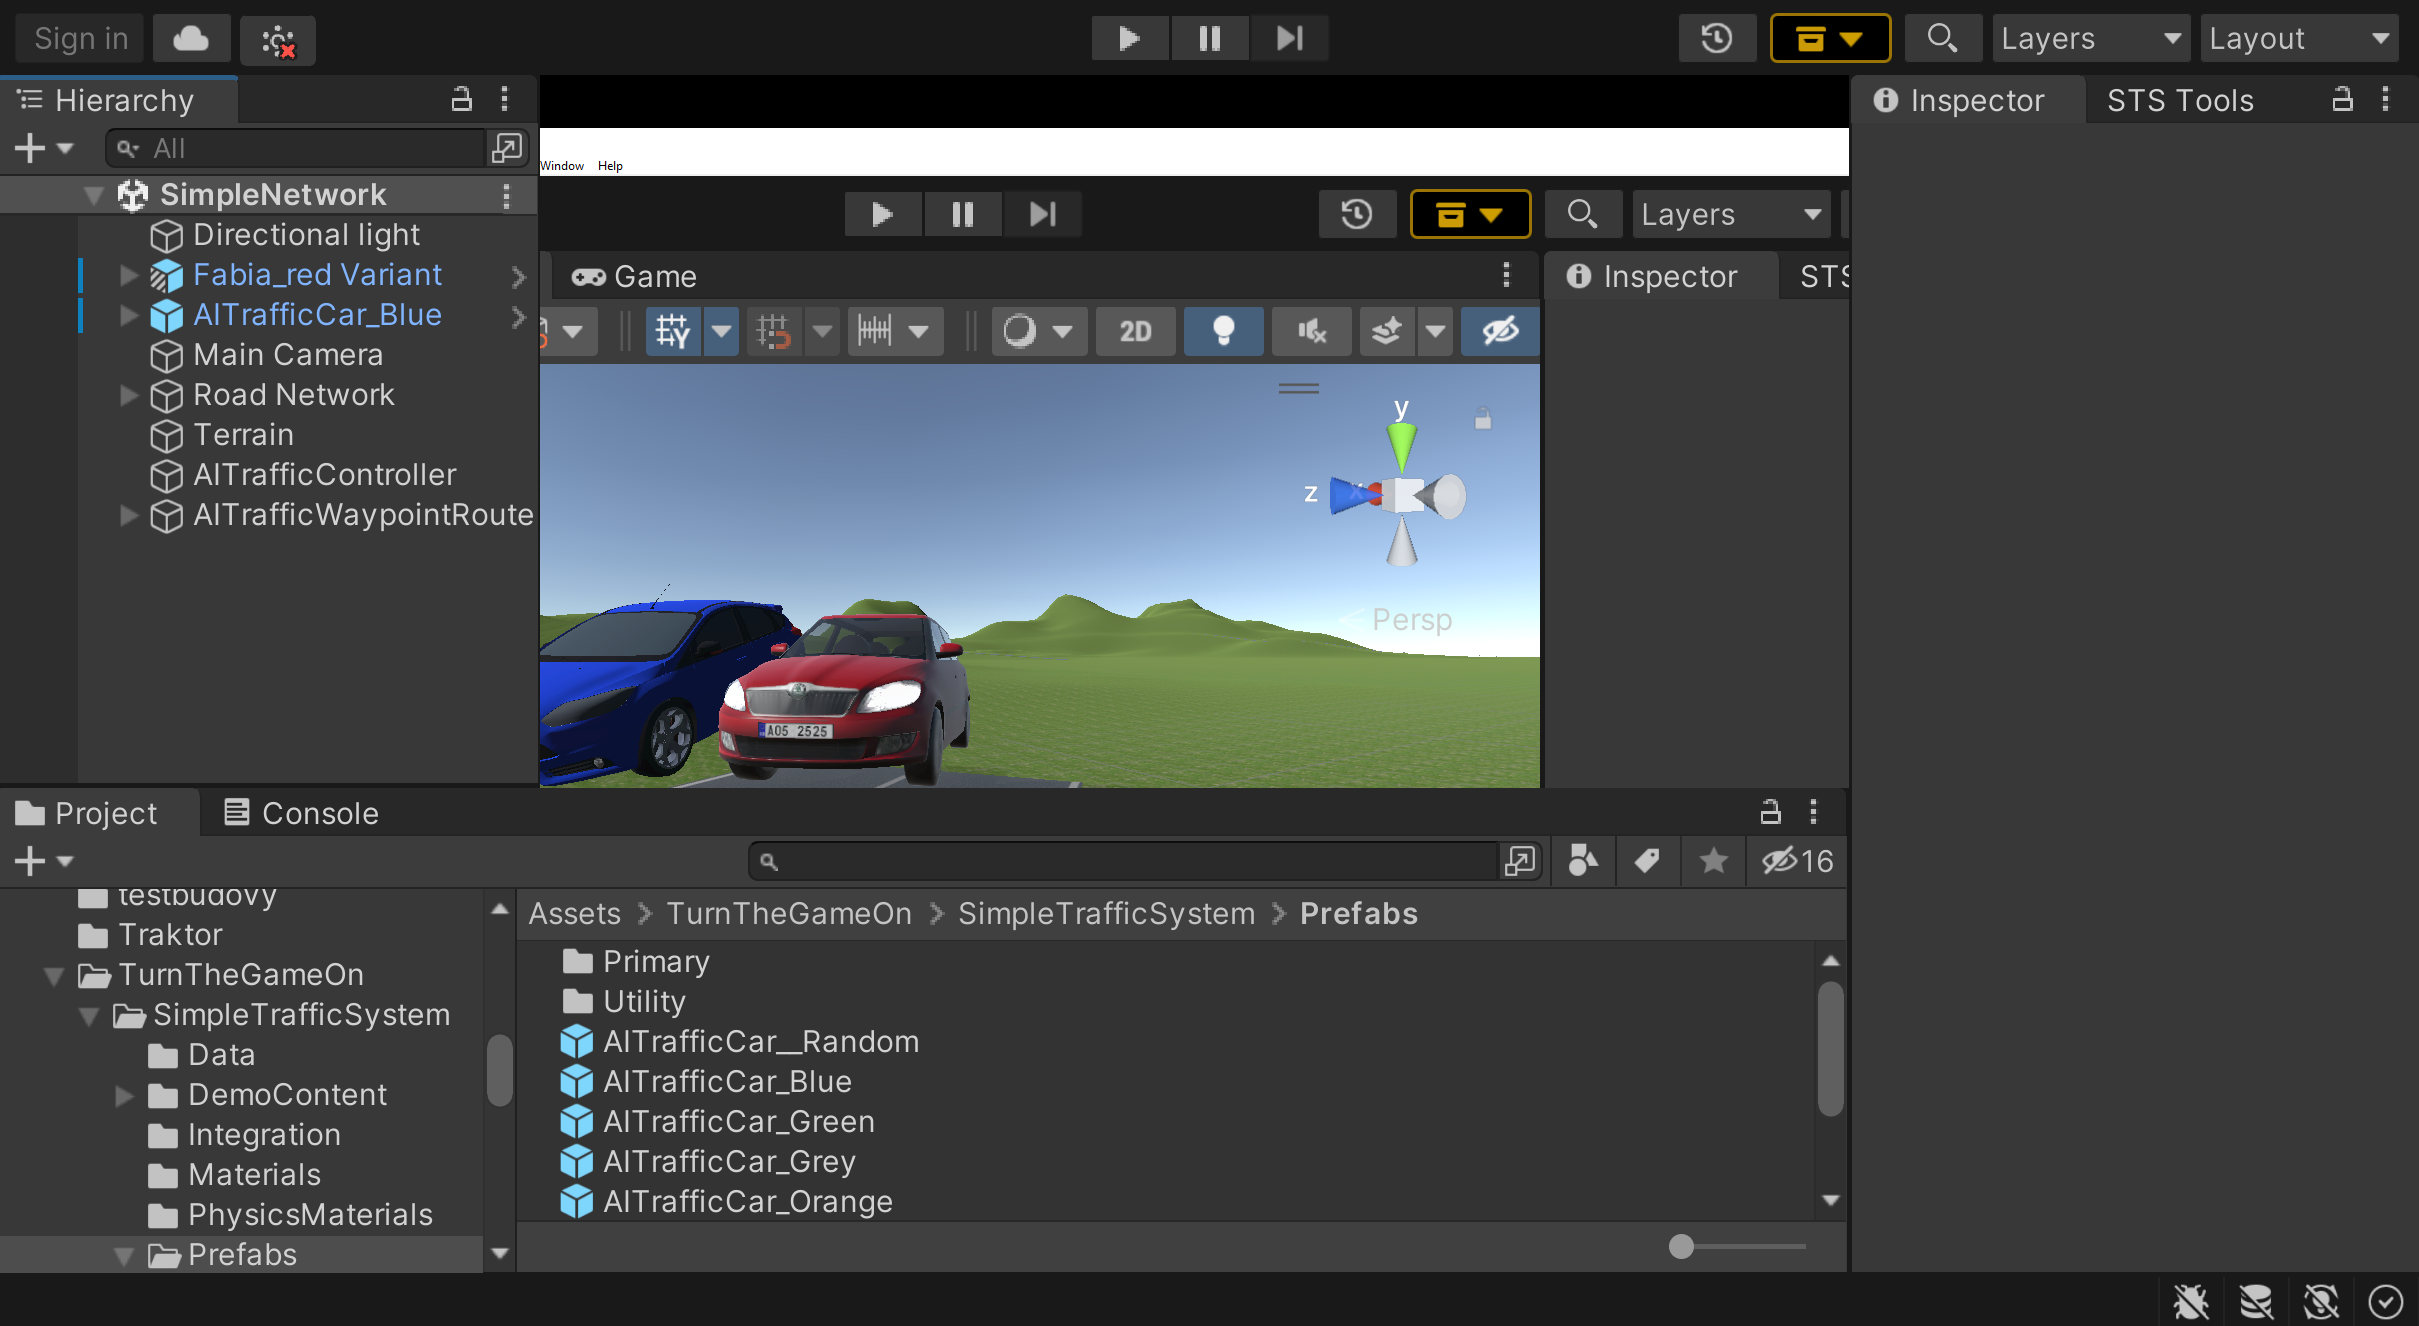
\includegraphics[width=.9\textwidth]{unityUI.png}
    \caption{The Unity development platform UI}
    \label{unity}
\end{figure}

\end{document}